\section{Testing instructions}
\label{sec:test}

When you get to Beerculator's web page, the first thing to do is to enter your personal informations. To do so, in the \guillemotleft{} User data \guillemotright{} tab ({\sc figure}~\ref{fig:userData}), in the first text box you have to indicate your weight in kilogramms. Then, you have to pick your gender in the list: male or female. Once you are done here, you should click on the \guillemotleft{} Save \guillemotright{} button.\\

\begin{figure}[H]
	\centering
   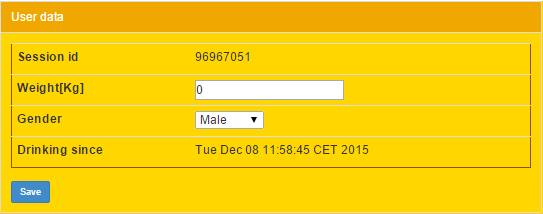
\includegraphics[scale=0.65]{./figures/userData.jpg}
   \caption{User data tab in the user interface of Beerculator}
   \label{fig:userData}
\end{figure}

After that, you can move on to the right side of the screen and start adding drinks to your list, in the \guillemotleft{} Drinks \guillemotright{} tab ({\sc figure}~\ref{fig:drinks}). To do so, you can click on the green squares corresponding to the drinks you have had. If you made a mistake, you can click on the associated red square in order to cancel and remove this drink. If you update your drinks this way, they are automatically saved. But you can also edit the quantity of each drink directly in the corresponding text box, which allows you to add or remove several drinks at the same time. If you do so, you should click on the \guillemotleft{} Save \guillemotright{} button. Also, if you want to cancel and start all over again, you can press the red \guillemotleft{} Reset \guillemotright{} button on the bottom of the page.\\

\begin{figure}[H]
	\centering
   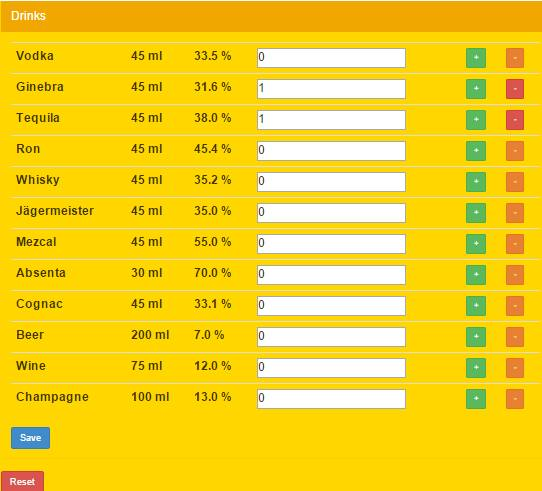
\includegraphics[scale=0.65]{./figures/drinks_tab.jpg}
   \caption{Drinks tab in the user interface of Beerculator}
   \label{fig:drinks}
\end{figure}

Then, you can launch the computation in the \guillemotleft{} Calculation \guillemotright{} tab ({\sc figure}~\ref{fig:calcul}) by clicking on the \guillemotleft{} Calculate \guillemotright{} button. The BAC value is indicated in the first text block, and it is followed by the number of hours before you get sober again.

\begin{figure}[H]
	\centering
   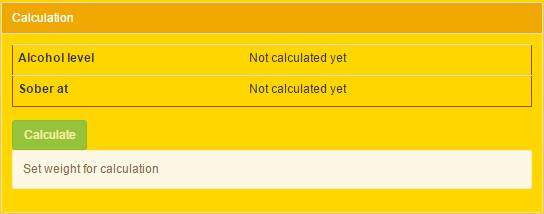
\includegraphics[scale=0.65]{./figures/calcul.jpg}
   \caption{Calculation tab in the user interface of Beerculator}
   \label{fig:calcul}
\end{figure}